%-------------------------------------------------------------------------------
%-------------------------------------------------------------------------------
%-------------------------------------------------------------------------------
\chapter{Listes}
%-------------------------------------------------------------------------------
%-------------------------------------------------------------------------------
\thispagestyle{empty}
%-------------------------------------------------------------------------------
%-------------------------------------------------------------------------------
{\sf Dans ce T.P. nous allons utiliser les listes comme variables, leur construction fera l'objet du sujet suivant.

La structure des fonctions à écrire sera souvent du même type :
\begin{lstlisting}
def une-fonction(var1, ..., varp, une_liste):
    n = len(une_liste)
    # Initialisations
    for i in range(n):
        # traitement pour chaque i
    # traitement global
    return le_resultat
\end{lstlisting}

Quand on n'a pas besoin de l'indice, Python permet la construction 
\begin{lstlisting}
def une-fonction(var1, ..., varp, une_liste):
    # Initialisations
    for x in une_liste:
        # traitement pour chaque x
    # traitement global
    return le_resultat
\end{lstlisting}

Plusieurs listes exemples sont données dans le fichier \type{TP06\_ex.py}
}
%-------------------------------------------------------------------------------
%-------------------------------------------------------------------------------
%-------------------------------------------------------------------------------
\section{Statistiques} 
%-------------------------------------------------------------------------------
%-------------------------------------------------------------------------------
%-------------------------------------------------------------------------------
\begin{Exercise}[title = Moyenne]
\it Écrire une fonction \type{moyenne(X)} qui calcule la moyenne des termes de la liste $X$ :

$\displaystyle \type{moyenne(X)} = \frac 1n \sum_{i=0}^n \type{X[i]}$ avec $n = \type{len(X)}$.

\type{moyenne(X0)} donne \type{1.9956097560975619}
\end{Exercise}
%-------------------------------------------------------------------------------
\begin{Answer}
\begin{lstlisting}
def moyenne(X):
    n = len(X)
    somme = 0
    for x in X:
        somme = somme + x
    return somme/n
\end{lstlisting}
\end{Answer}
%-------------------------------------------------------------------------------
%-------------------------------------------------------------------------------
\bigskip

La {\bf variance} d'une liste est définie par $\displaystyle \text{var}(X) =  \frac 1n \sum_{i=0}^n \bigl(\type{X[i]} -m_X\bigr)^2$ avec $m_X$ égal à la moyenne de la liste et $n = \type{len(X)}$.
%-------------------------------------------------------------------------------
%-------------------------------------------------------------------------------
\begin{Exercise}[title = Variance]
\it Écrire une fonction \type{var(X)} qui calcule la variance de la liste $X$.

On affectera la moyenne dans une variable avant la boucle pour éviter de répéter le même calcul.

\type{variance(Z0)} donne \type{6.558001189767997}
\end{Exercise}
%-------------------------------------------------------------------------------
\begin{Answer}
\begin{lstlisting}
def var(X):
    n = len(X)
    mX = moyenne(X)
    somme = 0
    for x in X:
        somme = somme + (x - mX)**2
    return somme/n
\end{lstlisting}
\end{Answer}
%-------------------------------------------------------------------------------
%-------------------------------------------------------------------------------
\bigskip

Si $X$ et $Y$ sont deux listes de même longueur, la {\bf covariance} de $X$ est $Y$ est 

$\displaystyle \text{cov}(X, Y) =  \frac 1n \sum_{i=0}^n \bigl(\type{X[i]} -m_X\bigr)\bigl(\type{Y[i]} -m_Y\bigr)$ avec $m_X$ égal à la moyenne de la liste $X$, $m_Y$ égal à la moyenne de la liste $Y$ et $n$ est la longueur commune de $X$ et de $Y$.

On pourra noter que $\text{var}(X) = \text{cov}(X, X)$
%-------------------------------------------------------------------------------
%-------------------------------------------------------------------------------
\begin{Exercise}[title = Covariance]
\it Écrire une fonction \type{cov(X, Y)} qui calcule la covariance des listes $X$ et $Y$.

Il sera nécessaire ici d'accéder aux éléments de \type{X} et \type{Y} par leurs indices.

\type{cov(T0, Y0)} donne \type{-1.6044390243902438}
\end{Exercise}
%-------------------------------------------------------------------------------
\begin{Answer}
\begin{lstlisting}
def cov(X, Y):
    n = len(X)
    mX = moyenne(X)
    mY = moyenne(Y)
    somme = 0
    for i in range(n):
        somme = somme + (X[i] - mX)*(Y[i] - mY)
    return somme/n
\end{lstlisting}
\end{Answer}
%-------------------------------------------------------------------------------
%-------------------------------------------------------------------------------
\bigskip


On admet que, $X$ et $Y$ sont deux listes de même longueur, alors la {\bf droite de régression} approchant $Y$ par rapport à $X$ est la droite d'équation $y = ax+b$ avec $m_Y = a.m_X + b$ et $a.\text{var}(X)=\text{cov}(X, Y)$.
%-------------------------------------------------------------------------------
%-------------------------------------------------------------------------------
\begin{Exercise}[title = Droite de régression]
\it Écrire une fonction \type{regression(X, Y)} qui calcule les coefficients$a$ et $b$ de la droite de régression de $X$ à $Y$.

\type{regression(X0, Y0)} donne \type{(2.2937900415993773, 1.7193194828375322)}
\end{Exercise}
%-------------------------------------------------------------------------------
\begin{Answer}
\begin{lstlisting}
def regression(X, Y):
    a = cov(X, Y)/var(X)
    b = moyenne(Y) - a*moyenne(X)
    return a, b
\end{lstlisting}
\end{Answer}
%-------------------------------------------------------------------------------
%-------------------------------------------------------------------------------
\subsection{Premiers graphes} 
%-------------------------------------------------------------------------------
%-------------------------------------------------------------------------------
Le module \type{matplotlib} permet de tracer des représentations de valeurs, c'est particulièrement utile dans le cas de listes. Nous utiliserons la sous-bibliothèque \type{pyplot} que l'on simplifiera par \type{plt}.
\begin{lstlisting}
import matplotlib.pyplot as plt
\end{lstlisting}

Il existe deux modes de tracé.
\begin{enumerate}
    \item Le mode standard construit les graphismes {\bf sans les afficher}, ils sont enrichis pas-à-pas. Quand toutes les instructions sont écrites, on demande l'affichage par \type{plt.show()} ; une fenêtre avec les graphismes apparaît et il faut la refermer pour continuer à utiliser Python. Nous utiliserons ce mode.
    \item Le mode interactif permet l'affichage de chaque commande en temps réel, sans monopoliser Python. Le principal inconvénient est que les graphismes deviennent vite surchargés, il faut régulièrement les effacer (\type{plt.clf()}). 
    \item On passe en mode interactif avec \type{plt.ion}, on en sort avec \type{plt.ioff}.
\end{enumerate}

\medskip

La fonction principale est \type{plt.plot}. Elle admet 2 utilisations.
\begin{enumerate}
    \item \type{plt.plot(X)} où \type{X} est une liste, relie les points de coordonnées \type{(i, X[i])} par des segments de droite, elle présente les valeurs de \type{X} dans l'ordre de la liste.
    \item \type{plt.plot(X, Y)} où \type{X} et \type{Y} sont deux listes {\bf de même longueur} relie les points de coordonnées \type{(X[i], Y[i])} par des segments de droite, elle présente les évolutions des les valeurs de \type{Y} en fonction de celles de \type{X}.
    \item Quand la liste n'est pas triée dans l'ordre croissant, la représentation ci-dessus n'est pas très signifiante. Parmi les nombreuses options de tracé, il existe la possibilité de représenter simplement les points sans tracer les segments avec un paramètre supplémentaire \type{'o'}, 
\end{enumerate}
%-------------------------------------------------------------------------------
\begin{center}
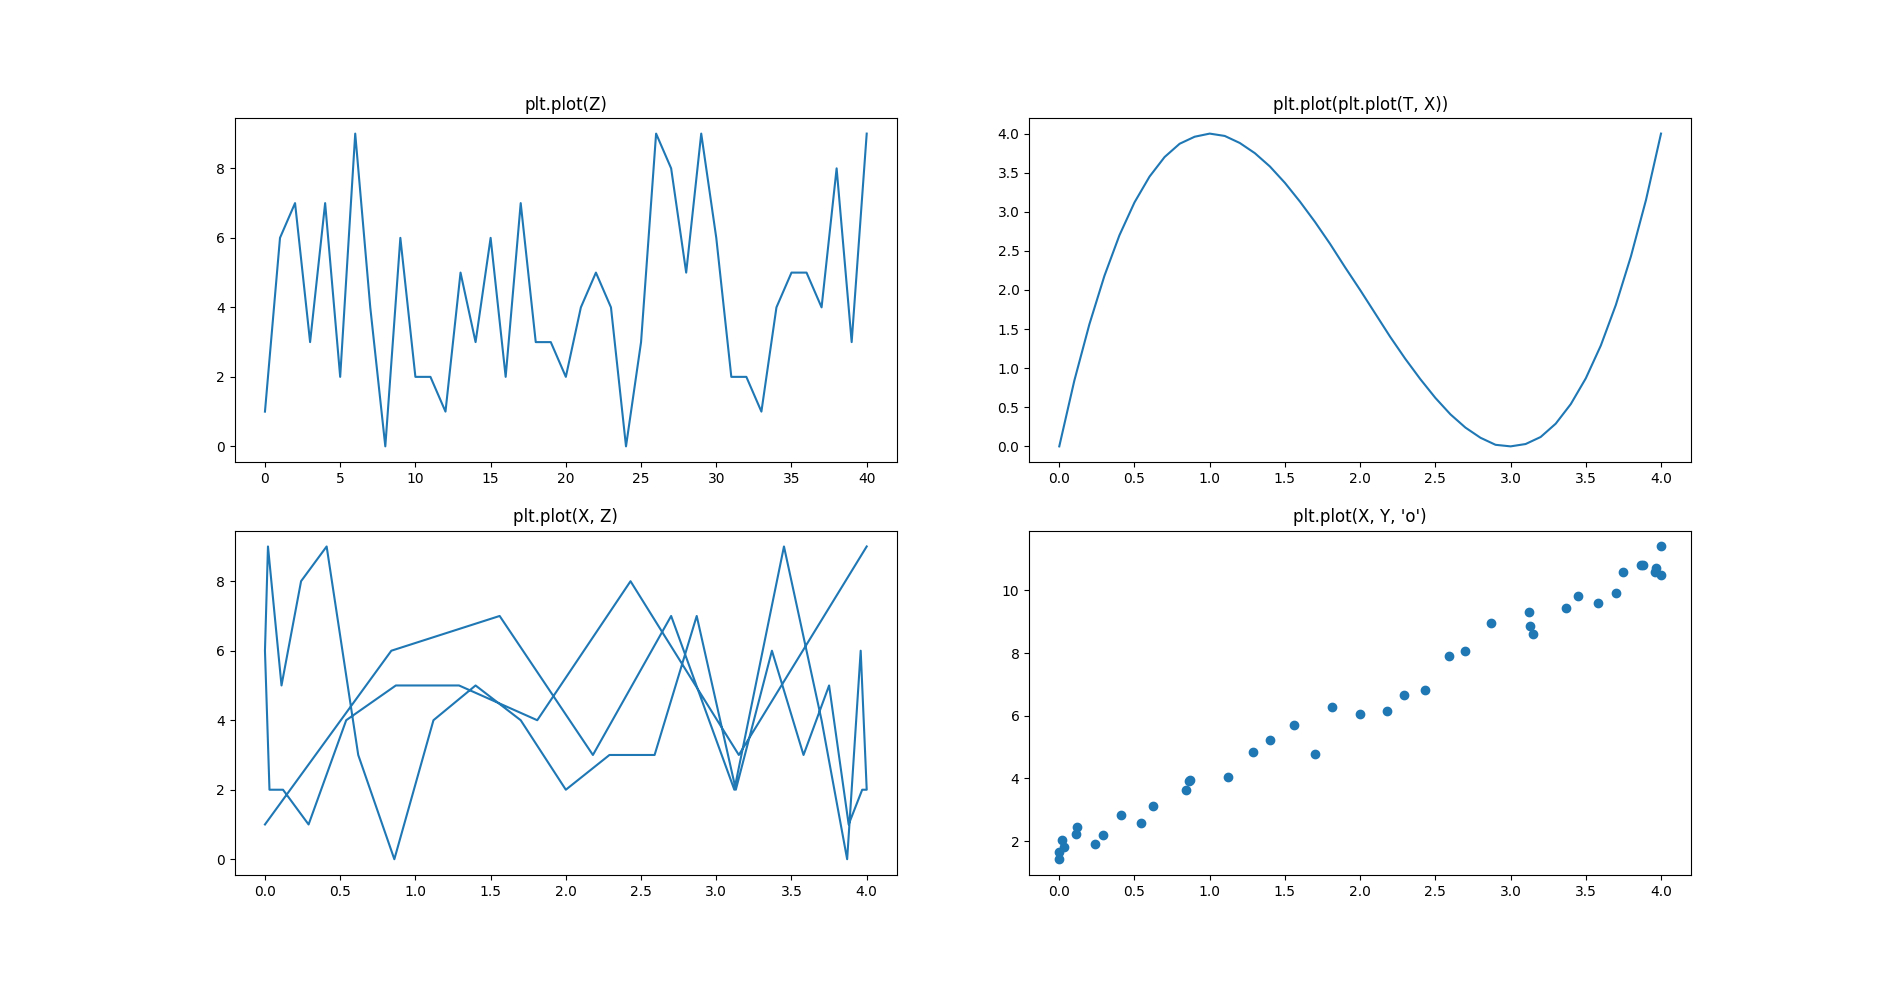
\includegraphics[width=1\linewidth]{TP06_plt.png} 
\end{center}
%-------------------------------------------------------------------------------

\vskip -1cm

On peut tracer plusieurs représentations (\type{plt.plot}) sur un même graphe.
%-------------------------------------------------------------------------------
%-------------------------------------------------------------------------------
\begin{Exercise}[title=Tracé de la droite de régression]
\it Après avoir calculé les coefficients ($a$ et $b$) de la droite de régression approchant \type{Y0} en fonction de \type{X0}, représenter sur un même graphe les points de coordonnées \type{(X0[i], Y0[i])} et la droite de régression. Pour tracer une droite d'équation $y = ax + b$ sur $[\alpha, \beta]$, on pourra tracer le segment entre les points $(\alpha, a.\alpha + b)$ et $(\beta, a.\beta + b)$.
\end{Exercise}
%-------------------------------------------------------------------------------
\begin{Answer}
\begin{lstlisting}
a, b = regression(X0, Y0)
c = a*4 + b
plt.plot(X0, Y0, 'o')
plt.plot([0, 4], [b, c])
plt.show()
\end{lstlisting}
%-------------------------------------------------------------------------------
\begin{center}
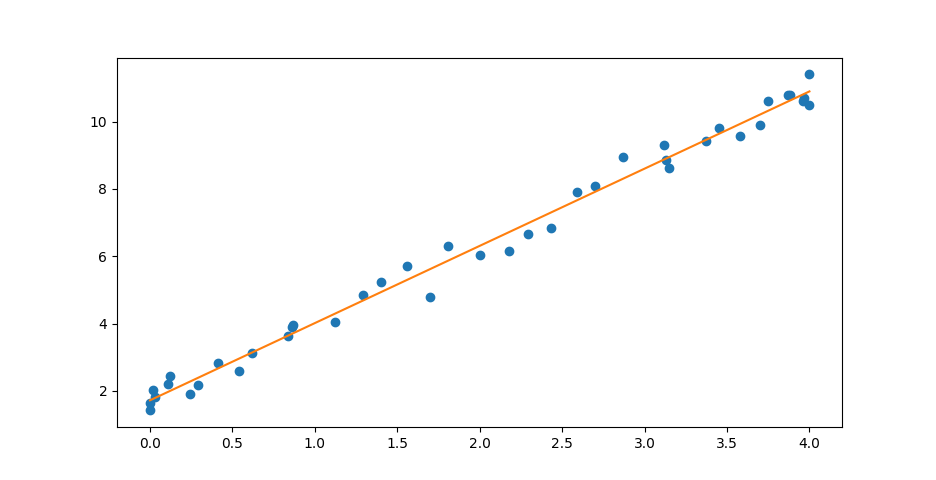
\includegraphics[width=1\linewidth]{TP06_ex05.png} 
\end{center}
%-------------------------------------------------------------------------------
\end{Answer}
%-------------------------------------------------------------------------------
%-------------------------------------------------------------------------------
%-------------------------------------------------------------------------------
\section{Tests} 
%-------------------------------------------------------------------------------
%-------------------------------------------------------------------------------
%-------------------------------------------------------------------------------
Lorsque l'on effectue un test sur une liste, on maintient une variable à valeur booléenne que l'on initialise avec une valeur qui est, en général, le résultat pour une liste vide. Par exemple, si on cherche si au moins un terme d'une liste est nul, le résultat initial est \type{False} : on n'a pas encore trouve de terme nul. On parcourt ensuite la liste et on transforme le résultat en \type{True} si on trouve un terme nul. Pour l'instant on ne cherchera pas à cesser la recherche dès qu'on a trouvé un terme nul.
\begin{lstlisting}
def contient0(liste):
     out = False
    for x in liste:
        if x == 0:
            out = True
    return out
\end{lstlisting}
On ne cherchera pas pour l'instant à optimiser les calculs et à renvoyer un résultat dès que le résultat est certain.
%-------------------------------------------------------------------------------
%-------------------------------------------------------------------------------
\begin{Exercise}[title=Positivité]\it
Tester la positivité d'une liste est ambigu : on peut tester s'il existe un élément positif ou si tous les éléments sont positifs.

Ici positif signifie positif ou nul.
%-------------------------------------------------------------------------------
\begin{enumerate}
    \item Écrire une fonction \type{tout\_positif(liste)} qui renvoie \type{True} ou \type{False} selon que tous les éléments de la liste sont positifs ou non.
    \item Écrire une fonction \type{existe\_positif(liste)} qui renvoie \type{True} s'il existe au moins un élément positif dans la liste et \type{False} sinon.
\end{enumerate}
%-------------------------------------------------------------------------------
\end{Exercise}
%-------------------------------------------------------------------------------
\begin{Answer}
L'initialisation est différente.
%-------------------------------------------------------------------------------
\begin{enumerate}
\item  Si on cherche à savoir si tous les éléments sont positifs la réponse est \type{True} jusqu'à ce qu'on trouve un élément négatif. Il est important de ne pas remettre le résultat à \type{True} si on retrouve une valeur positive, il n'y a pas de traitement \type{else}.
\begin{lstlisting}
def tout_positif(liste):
               False sinon"""
    resultat = True
    for x in liste:
        if x < 0:
            resultat = False
    return resultat
\end{lstlisting}
%-------------------------------------------------------------------------------
\item Ici la réponse est \type{False} jusqu'à preuve du contraire.
\begin{lstlisting}
def existe_positif(liste):
    resultat = False
    for x in liste:
        if x >= 0:
            resultat = True
    return resultat
\end{lstlisting}
\end{enumerate}
%-------------------------------------------------------------------------------
\end{Answer}
%-------------------------------------------------------------------------------
%-------------------------------------------------------------------------------
\begin{Exercise}[title=Croissance]\it
Écrire une fonction \type{croissante(liste)} qui renvoie \type{True} ou \type{False} selon que les termes de la liste forme une suite croissante ou non.

\type{croissance(T0)} donne \type{True}, 
\type{croissance(X0)} donne \type{False}
%-------------------------------------------------------------------------------
\end{Exercise}
%-------------------------------------------------------------------------------
\begin{Answer}
%-------------------------------------------------------------------------------
\begin{lstlisting}
def croissante(liste):
    n = len(liste)
    resultat = True
    for i in range(n-1):
        if liste[i] > liste[i+1]:
            resultat = False
    return resultat
\end{lstlisting}
%-------------------------------------------------------------------------------
\newpage
\end{Answer}
%-------------------------------------------------------------------------------
%-------------------------------------------------------------------------------
%-------------------------------------------------------------------------------
\section{Maximums} 
%-------------------------------------------------------------------------------
%-------------------------------------------------------------------------------
%-------------------------------------------------------------------------------
La recherche du maximum d'une expression dépendant des termes d'une liste doit être initialisée avec soin ; par exemple, il ne faut pas initialiser le maximum des termes d'une liste par 0 et rechercher les termes qui dépassent car il se peut que tous les termes soient négatifs. L'initialisation d'un maximum doit être une valeur possible de l'expression.

\begin{lstlisting}
def maximum(liste):
    maxi = liste[0]
    for x in liste:
        if x > maxi:
            maxi = x
    return maxi
\end{lstlisting}
%-------------------------------------------------------------------------------
%-------------------------------------------------------------------------------
\begin{Exercise}[title =Minimum]
\it Écrire une fonction \type{minimum(liste)} qui calcule le minimum d'une liste non vide.

\type{minimum(Y0)} donne \type{1.42}
\end{Exercise}
%-------------------------------------------------------------------------------
\begin{Answer}
\begin{lstlisting}
def minimum(liste):
    mini = liste[0]
    for x in liste:
        if x < mini:
            mini = x
    return mini
\end{lstlisting}
%-------------------------------------------------------------------------------
\end{Answer}
%-------------------------------------------------------------------------------
%-------------------------------------------------------------------------------
\begin{Exercise}[title=Indice du maximum]
\it Écrire une fonction \type{indiceMax(liste)} qui calcule un indice en lequel une liste non vide atteint son maximum. 
Si la liste atteint son maximum plusieurs fois, quel indice votre fonction renvoie-t-elle ?

\type{indiceMax(Z0)} donne \type{6} ou \type{40}.
\end{Exercise}
%-------------------------------------------------------------------------------
\begin{Answer}
\begin{lstlisting}
def indiceMax(liste):
    n = len(liste)
    i_maxi = 0
    for i in range(1, n):
        if liste[i] > liste[i_max]:
            i_max = i
    return i_max
\end{lstlisting}
%-------------------------------------------------------------------------------
L'indice renvoyé est le premier en lequel la liste atteint son maximum.

Si on remplace le test par \type{if liste[i] >= liste[i\_max]:}, ce sera le dernier indice.
\end{Answer}
%-------------------------------------------------------------------------------
%-------------------------------------------------------------------------------
\begin{Exercise}[title=Sommes de 3 termes]
\it Écrire une fonction \type{maximum3(liste)} qui calcule le maximum de la somme de 3 termes consécutifs d'une liste de longueur au moins 3.

\type{maximum3(X0)} donne \type{11.93}
\end{Exercise}
%-------------------------------------------------------------------------------
\begin{Answer}
\begin{lstlisting}
def maximum3(liste):
    n = len(liste):
    max3 = liste[0] + liste[1] + liste[2]
    for i in range(1, n-2):
        s3 = liste[i] + liste[i+1] + liste[i+2]
        if s3 > max3:
            max3 = s3
    return max3
\end{lstlisting}
%-------------------------------------------------------------------------------
\end{Answer}
%-------------------------------------------------------------------------------
%-------------------------------------------------------------------------------
\begin{Exercise}[title=Deuxième valeur]
\it Écrire une fonction \type{second(liste)} qui calcule le deuxième plus grand terme d'une liste de nombres. En cas d'ex-æquo pour le maximum, la fonction peut renvoyer le maximum.

\type{second(Y0)} donne \type{10.8}, \type{second(Z0)} donne \type{9}
\end{Exercise}
%-------------------------------------------------------------------------------
\begin{Answer}
\begin{lstlisting}
def second(liste):
    n = len(liste)
    max1 = max(liste[0], liste[1])
    max2 = mini(liste[0], liste[1])
    for i in range(2, n):
        x = liste[i]
        if x > max1:
            max2 = max1
            max1 = x
        elif x > max2:
            max2 = x
    return max2
\end{lstlisting}
%-------------------------------------------------------------------------------
\end{Answer}
%-------------------------------------------------------------------------------
%-------------------------------------------------------------------------------

\medskip

L'augmentation maximale d'une liste est le plus grand accroissement \type{liste[j] - liste[i]} pour $i \le j$. Sa valeur est toujours positive et vaut 0 dans le cas d'une liste décroissante. L'augmentation maximale est donc, en notant $L_i$ la valeur de \type{liste[i]} et $n$ est la longueur de la liste,
\[\text{augMax} = \max\left\{L_j - L_i\ ;\ 0\le i \le j < n\right\}\]
%-------------------------------------------------------------------------------
%-------------------------------------------------------------------------------
\begin{Exercise}[title=Augmentation maximale]
\it  Écrire une fonction \type{augMax(liste)} qui calcule l'augmentation maximale d'une liste de nombres. 

\type{augMax(Y0)} donne \type{9.76}
\end{Exercise}
%-------------------------------------------------------------------------------
\begin{Answer} On ne recalcule pas \type{liste[i] - liste[i]}
\begin{lstlisting}
def augMax(liste):
    n = len(liste)
    augM = 0
    for i in range(n-1):
        for j in range(i, n):
            aug = liste[j] - liste[i]
            if aug > augM:
                augM = aug
    return augM
\end{lstlisting}
%-------------------------------------------------------------------------------
\newpage
\end{Answer}
%-------------------------------------------------------------------------------
%-------------------------------------------------------------------------------
\begin{Exercise}[title={En plus}, difficulty = 2]
\it  
\begin{enumerate}
    \item Écrire une fonction \type{second(liste)} qui calcule la deuxième valeur d'une liste, distincte du maximum, sauf dans le cas d'une liste constante.
    \item Écrire une fonction \type{majoritaire(liste)} qui calcule l'élément majoritaire d'une liste {\bf triée} avec une unique boucle \type{for}. Que compte la fonction si la liste n'est pas triée ?
    \item Écrire une fonction \type{pivot(liste)} qui renvoie un indice $i$ tel que $\displaystyle \left|\sum_{k=0}^{i-1}L_k-\sum_{k=i}^{n-1}L_k\right|$ est minimale : on veut couper la liste en deux parties de sommes presqu'égales.
    \item Écrire une fonction \type{augMax(liste)} qui n'utilise qu'une boucle \type{for}.
    \item Écrire une fonction qui calcule la somme maximale d'une tranche de liste (suite de termes consécutifs) en n'employant qu'une boucle \type{for}.
\end{enumerate}
\end{Exercise}
%-------------------------------------------------------------------------------
\begin{Answer} 
\begin{enumerate}
\item Il faut gérer les cas d'égalité.
\begin{lstlisting}
def second(liste):
    n = len(liste)
    max1 = liste[0]
    max2 = liste[0]
    for i in range(1, n):
        x = liste[i]
        if x > max1:
            max2 = max1
            max1 = x
        elif (max1 == max2 > x) or (max1 > x > max2):
            max2 = x
    return max2
\end{lstlisting}

\item Si la liste n'est pas triée, on renvoie l'élément le plus répété.
\begin{lstlisting}
def majoritaire(liste):
    n = len(liste)
    nb_maj = 1
    maj = liste[0]
    encours = 1
    for i in range(1, n):
        if liste[i] == liste[i-1]:
            encours += 1
            if encours > nb_maj:
                nb_maj = encours
                maj = liste[i]
        else:
            encours = 1
    return maj
\end{lstlisting}

\item Pour chaque $i$ on calcule les deux sommes qu'il sépare. On peut le faire avec une addition et une soustraction à chaque étape. On notera qu'il y a $n+1$ résultats possibles : de 0 à $n$.
\begin{lstlisting}
def pivot(liste):
    n = len(liste)
    gauche = 0
    droite = 0
    for x in liste:
        droite = droite + x
    e_min = abs(droite - gauche)
    i_min = 0
    for i in range(n):
        x= liste[i]
        gauche = gauche + x
        droite = droite - x
        e = abs(gauche - droite)
        if e < e_min:
           e_min = e
           i_min = i + 1
    return i_min
\end{lstlisting}
\type{pivot([1, 2, 3, 6])} donne \type{3}

\newpage

\item On remarque que le maximum d'un écart qui finit en $j$ est la différence entre $L_j$ et le minimum jusqu'à $j$ : il suffit donc de calculer ce minimum dans la boucle.
\begin{lstlisting}
def augMax(liste):
    n = len(liste)
    augM = 0
    mini = liste[0]
    for i in range(1, n):
        mini = min(mini, liste[i])
        aug = liste[i] - mini
        if aug > augM:
            augM = aug
    return augM
\end{lstlisting}

\item C'est presque l'exercice précédent : on veut le minimum des $\displaystyle \sum_{k=i}^j L_k$ pour $0\le i \le j < n$. Si on pose $\displaystyle S_i = \sum_{k=0}^j L_k$ et $S_{-1} = 0$, on veut le minimum des $S_j-S_{i-1}$.
\begin{lstlisting}
def trancheMax(liste):
    n = len(liste)
    tMax = 0
    sMin = 0
    S = 0
    for i in range(n):
        S = S + liste[i]
        t = S - sMin
        if t > tMax:
            tMax = t
        sMin = min(sMin, S)
    return tMax
\end{lstlisting}
\type{trancheMax([2, -1, 3, -3, 2])} donne \type{4}
\end{enumerate}

%-------------------------------------------------------------------------------
\end{Answer}
%-------------------------------------------------------------------------------
%-------------------------------------------------------------------------------


